\chapter{Application Specific Dataflow for Weather Codes}



\section{GPU Approach}



\section{Our Approach: Deep Pipelining}


\section{Example}
Comment: At the end of this chapter, try to again have a transition into the next chapter by presenting the challenge of determining how to lay out the buffers.



%This seems like it will become a very small chapter. If they were sections like in a paper, that would be OK, but these chapters indicate a significant portion of the thesis. Maybe we can reevaluate and possibly merge later.

\section{{Why we think reconfigurable architectures are the way to go.}}




\begin{figure}[h]
	\centering
	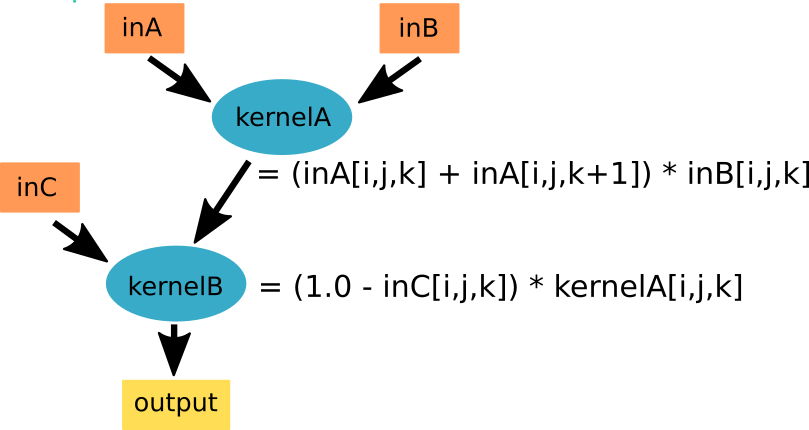
\includegraphics[width=1.0\textwidth]{drawings/approach-stencil-program.png}
	\caption{Example stencil program in high-level data flow representation.}
	\label{fig:mesh1}
\end{figure}

\begin{figure}[h]
	\centering
	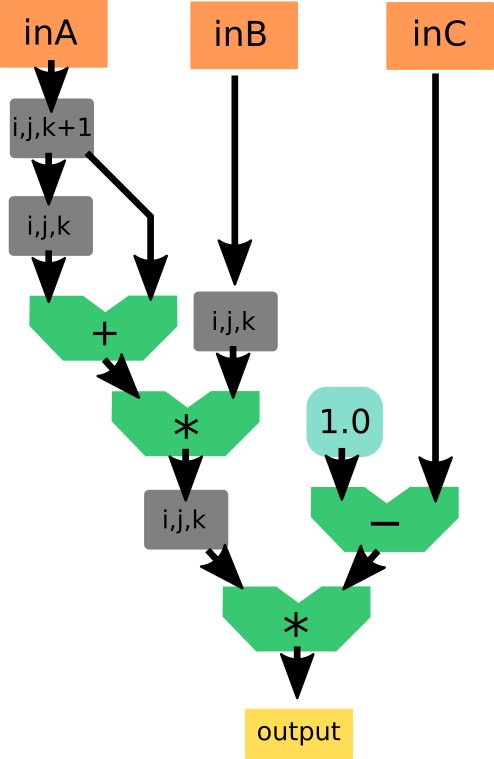
\includegraphics[width=1.0\textwidth]{drawings/approach-stencil-program-pipeline.png}
	\caption{Example stencil program visualized as a pipeline.}
	\label{fig:mesh1}
\end{figure}

\begin{figure}[h]
	\centering
	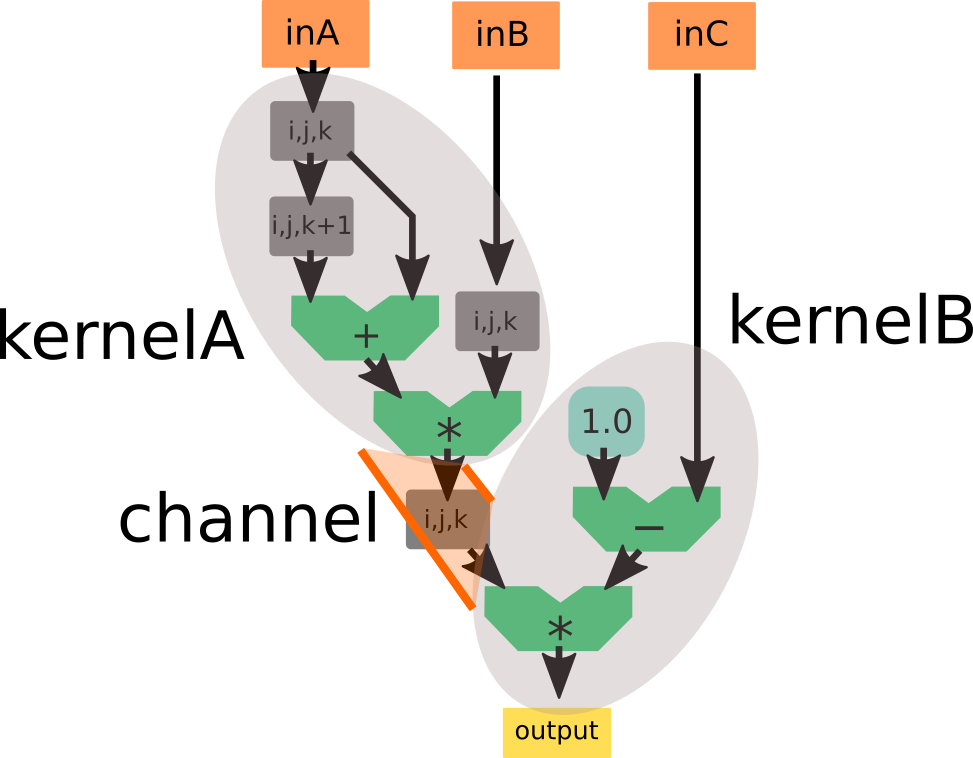
\includegraphics[width=1.0\textwidth]{drawings/approach-stencil-program-pipeline-annotated.png}
	\caption{Example stencil program with additional annotation about the structure of kernels and channels connecting the kernels.}
	\label{fig:mesh1}
\end{figure}